\documentclass[12pt]{article}
\usepackage{geometry}                % See geometry.pdf to learn the layout options. There are lots.
\geometry{letterpaper}                   % ... or a4paper or a5paper or ... 
%\geometry{landscape}                % Activate for for rotated page geometry
\usepackage[parfill]{parskip}    % Activate to begin paragraphs with an empty line rather than an indent
\usepackage{daves,fancyhdr,natbib,graphicx,dcolumn,amsmath,lastpage,url}
\usepackage{amsmath,amssymb,epstopdf,longtable}
\usepackage[final]{pdfpages}
\DeclareGraphicsRule{.tif}{png}{.png}{`convert #1 `dirname #1`/`basename #1 .tif`.png}
\pagestyle{fancy}
\lhead{CE 3372 WATER SYSTEMS DESIGN}
\rhead{FALL 2018 - SEC 001\&002 (T-TH)}
\lfoot{}
\cfoot{}
\rfoot{Page \thepage\ of \pageref{LastPage}}
\renewcommand\headrulewidth{0pt}



\begin{document}
\section*{Syllabus}

%%%%%% BEGIN SYLLABUS COMPONENT %%%%%%%%%%%%%%%%%%%%%%%%%%%%%%%%%%%%%2010-0814TGC%%%%%%%%%%%%%%%%%%%%%%%%%%%%%%%%%%%%%%%%%
\subsection*{{Course Location, Textbook, Instructor Contact Information}}
\begin{tabular}{p{1.5in}p{5.0in}}
Class Meetings:  &    18:30-19:50 , T-TH, CE 001 (Section 001) \\
~ &    11:00-12:20 , T-TH, CE 211 (Section 002) \\
Instructor: & Theodore G. Cleveland, CE Room 203F \\
TA: & none \\
Office Hours: & Open Door Policy \\
%~ & T. Cleveland MW 08:00 - 10:00 \\
Telephone: & (806) 834-5101 \\
%Cell Phone: & (832) 722-4185 (more reliable than office phone) \\
E-mail: & \texttt{theodore.cleveland@ttu.edu}\\
Web: & \texttt{http://54.243.252.9/ce-5366-webroot/} \\
%%%%%%2010-0814TGC%%%%%%%%%%%%%%%%%%%%%%%%%%%%%%%%%%%%%%%%%
Textbook(s) : &  ~ \\ 
~ & Water Resources Systems Planning and Management (WRPM) \citep{UNESCO2005}\\
~ & Principles of Integrated Water Resources Management (IWRM) \citep{UNESCO-IHE2014}\\
%\cite{mays2011} \\
%~ & \cite{ncees2008} & \cite{rossman2000} & \cite{rossman2009} \\
%~ & \cite{gironas2009} & and more ... & \\
 %\cite{cleveland2013} \\
 %%%%%%2010-0814TGC%%%%%%%%%%%%%%%%%%%%%%%%%%%%%%%%%%%%%%%%%
Copyright : & \textsl{Copyright $\copyright$ 2018 Theodore G. Cleveland, all rights reserved.} \\
\end{tabular}
%%%%%%2010-0814TGC%%%%%%%%%%%%%%%%%%%%%%%%%%%%%%%%%%%%%%%%%
\subsection*{{Catalog Description}}
\begin{quote} \textbf{CE 5366: Water Resources Management (3:3:0)} 
Models and other technical elements of water resources systems in context of the political, social, and other environments in which they exist.
\end{quote}
%%%%%%2010-0814TGC%%%%%%%%%%%%%%%%%%%%%%%%%%%%%%%%%%%%%%%%%
%%%%%%%%%%%%%%%%%%%%%%%%%%%%%%%%%%%%%%%%%%%%%%%%%%%%%%%
%%%%%%%%%%%%%%%%%%%%%%%%%%%%%%%%%%%%%%%%%%%%%%%%%%%%%%%
\subsection*{{Course Objectives}}
The purpose of this class is to study ...
\begin{enumerate}
\item Construct solution tools using \textbf{R} as a computation engine and \textbf{Excel} as an interface for small-scale linear and non-linear programming problems.
\item Locate and use solution tools for large-scale linear and non-linear programming problems.
\item Formulate integrated simulation and optimization models for improved decision making and analysis in water resources management.
\item Quantify risks and uncertainties in planning, design, and management objective(s) in water resources systems. 
\item Evaluate alternatives in water resources management with respect to economic, environmental, ecological, regulatory, and social aspects. 
\item Describe the large scale complex interactions between engineered infrastructure and natural systems and the issues associated with holistic decision-making.
\end{enumerate}

\subsection*{ABET Program Outcomes}
A subset of the ABET Program Outcomes are addressed in CE 3372, these outcomes are listed below:\footnote{Item 3[b] below is only partially fulfilled --- in this course students will analyze and interpret data, design of experiments is beyond the scope of the class.}


\begin{tabular}{p{0.5in}p{5.5in}}
\texttt{3[a].}  & Ability to apply knowledge of mathematics, science, and engineering.\\
\texttt{3[b].}  & Ability to design and conduct experiments, as well as to analyze and interpret data.\\
\texttt{3[e].}  & Ability to identify, formulate, and solve engineering problems.\\
\texttt{3[i].}   & Recognition of need for life-long learning.\\
\texttt{3[k].}  & Ability to use the techniques, skills, and modern engineering tools necessary for engineering practice.\\
\texttt{8[d].}  & Proficiency in water resources engineering.\\
\end{tabular}
%\newpage



\section*{Course Specific Policies}
Any  policies stated in this section that differ from University Operating Policies are null and void and the University Operating Policies shall be in force.
\subsection*{Disability:}
Texas Tech policy provided as part of syllabus (see last section).

%\textsl{ "Any student who, because of a disability, may require special arrangements in order to meet
%the course requirements should contact the instructor as soon as possible to make any necessary arrangements.
%Students should present appropriate verification from Student Disability Services during the instructors office hours. Please note instructors are not allowed to provide classroom accommodations
%to a student until appropriate verification from Student Disability Services has been provided.
%For additional information, you may contact the Student Disability Services office at 335 West Hall or
%806- 742-2405."}

\subsection*{Religious Holidays:}
\textsl{ "A student who intends to observe a religious holy day (as defined by OP 34.19) should
make that intention known to the instructor prior to the absence in order to receive accommodations
prescribed by OP 34.19."}

\subsection*{Cellphones/Pagers: }
Please set your personal communication devices to silent ring or off during class. 
Do not take calls in class. Disturbance during class time is not acceptable.

\subsection*{Prerequisites:} 
Mastery of material from CE 3305 and CE 3354 or equivalent is expected.

\subsection*{Attendance:} Roll will be taken to determine attendance for class participation.  Please let the instructor know in advance if you must miss a class for a legitimate reason\footnote{Legitimate reasons include: Academically-related extracurricular activities (ASCE, AGU, etc.); Illness with documentation; Federal Family Leave Act Policies; Orders to activate (Military, Peace Officer, Public Health, etc.).  Bring me some kind of documentation for such absences.}. 

\section*{Evaluation Instruments and Grading}
Student performance will be evaluated using attendance (coming to class), article reviews, exercises (homework), project reports, and examinations.   The exams will derive much of their content from the exercises.  %At the end of the semester students are to turn in a portfolio of all graded work.  The portfolio should be comprised of photocopies of exercise materials, article reviews, and exams 1 and 2.  The project report should be submitted under separate cover.  The portfolio should be bound using a binder clip.  The portfolio will not be returned.  

%\subsection*{Article Reviews:} 
%Several article reviews are assigned; part of professional development is reading and interpreting professional literature.  Due dates for these reviews are shown in Table \ref{tab:fall2013schedule}.  These reviews are shown as \texttt{R-\#}.

\subsection*{Exercises:} 
Assignments follow nearly every lecture and are due the following class meeting (but consult the schedule below for actual due dates -- changes are announced on the main page of the class website)\footnote{Legibility, correct method, and correct answer are substantial components of grading criteria.   The grader will not diagnose sources of arithmetic or algebra errors unless the errors are obvious.  Solutions are reviewed in class and posted on the server}.
\begin{enumerate}
\item Every homework assignment is to be accompanied by a descriptive memorandum containing your analysis
of the problem. 
Report materials should be prepared with a word processor. 
Hand computations may be turned in on engineering paper attached as an appendix to the memorandum\footnote{Regular binder paper is not acceptable --- use engineering paper.}; important steps in each solution must be shown. 
Legibility is determined by the reader; illegible materials will not be graded.
\item Assignments are to be uploaded to the learning management system (LMS) on the assigned date.\footnote{The use of a LMS (Learning Management System) is an experiment this semester.  The LMS is accessed through the course server.  If the LMS is not working, then assignments are due by midnight on the due date. Late assignments are not accepted.}
\item Due dates are shown in Table \ref{tab:fall2013scheduleA};  Exercises are denoted by \texttt{ES-\#}
\end{enumerate}

\subsection*{Engineering Reports:}  
A project report comprised of various components developed during the course is to be completed.  
The project is introduced early in the semester and is related to the design of a water distribution, stormwater collection, and/or wastewater collection system and accompanying appurtenances.    
There are two "reports" on the schedule: \texttt{RP-1}, and \texttt{RP-2}.  
The reports are to be constructed as a team activity (teams will be selected in the first two weeks of the semester).

\subsection*{Presentations}
An engineering presentation is to be completed and presented to the class for peer evaluation. 
The topic is the same as in \texttt{RP-2}.   The report is due by each team on the day of presentation.

\subsection*{Exams:} Two examinations will be given, they will be of approximately equal difficulty.
\begin{enumerate}
\item Examinations are open notes.
\item Examinations are comprehensive, even though the main focus will be the materials discussed prior to the examination.
\item Full credit for problems will only be given if all computations are documented.
\item Examination dates are shown in Table \ref{tab:fall2013scheduleA}.
\end{enumerate}

\section*{Grading:} Final grades are determined based on performance during the semester.  Letter grades will be assigned using University standards.  The \textbf{approximate} weighting of graded material in determining the final grade is as follows\footnote{Graded materials with fewer than 100 points will have raw scores recorded and will be normalized to 100 points for calculating the final grade.}
% Requires the booktabs if the memoir class is not being used
\begin{table}[h!]
   \centering
   \begin{tabular}{l l}
Item & Percent of Grade \\
\hline
\hline
Attendance and Participation & ~5\% \\
Project Presentation & ~5\% \\
Project Report-1 & ~10\% \\
Project Report-2 & ~10\% \\
Exercises & 20\% \\
Mid-Term Exam & 25\% \\
Final Exam & 25\% \\
\hline
\end{tabular}
\end{table}

\clearpage
\section*{Schedule}
\begin{center}
\begin{table}[ht!]
% \caption{Fall 2018 Course Schedule}
   \begin{tabular}{| p{0.8in} | p{3.4in} | p{2.0in} |} 
\hline
\hline
DATE & TOPIC & READINGS  \\
\hline
\hline
\texttt{01JUL24} & Water Resources Planning and Management & WRPM(pp.3-39) IWRM(pp.1-26)  \\
\texttt{02JUL24} & Decision Making and Uncertainty &   WRPM(pp.231-254) ~~~~ \\
\texttt{03JUL24} & Economics as Decision Support Structure & \cite{JamesLee1971} ~~~~\\
\texttt{04JUL24} & Independence Day (US Holiday) &   \\
\texttt{05JUL24} & Simulation Modeling for Decision Support  & WRPM(pp.59-80)  \\
\hline
\hline
\texttt{08JUL24} & Optimization Modeling for Decision Support  & WRPM(pp.81-134)  \\
\texttt{09JUL24} & Merit (Objective) Functions & WRPM(pp.293-308)  \\
\texttt{10JUL24} & Estimating Demand & Self-Study  \\
\texttt{11JUL24} & EPANET Introduction & Self-Study  \\
\texttt{12JUL24} & EPANET Examples & Self-Study  \\
\hline
\hline
\texttt{15JUL24} & Open Channels (Normal Flow) & Lesson-11   \\
\texttt{16JUL24} & Open Channels (Gradually Varied Flow) & Lesson-12 \\
\texttt{17JUL24} & SWMM Introduction & Lesson-13 9 \\
\texttt{18JUL24} & SWMM Examples & Lesson-14 \\
\texttt{19JUL24} & Hydrology - IDF For Preliminary Design & Lesson-15  \\
\hline
\hline
\texttt{22JUL24} & Inlet Hydraulics & Lesson-16  \\
\texttt{23JUL24} & By-Hand Rational Design & Lesson-17  \\
\texttt{24JUL24} & Goodwin Street Example & Lesson-18  \\
\texttt{25JUL24} & Tanglewilde Example & Lesson-19  \\
\texttt{26JUL24} & Hydrology - Design Storms & Lesson-20  \\
\hline
\hline
\texttt{29JUL24} & Hydraulic Check using SWMM & Lesson-21  \\
\texttt{30JUL24} & Dual Drainage Systems in SWMM & Lesson-22  \\
\texttt{31JUL24} & Detention Ponds & Lesson-23  \\

\hline
\hline
   \end{tabular}
   \label{tab:fall2013scheduleA}
\end{table}
\end{center}
\clearpage
\begin{thebibliography}{}

  
\bibitem[\protect\citeauthoryear{UNESCO}{UNESCO}{2005}]{UNESCO2005}
UNESCO (2005).
\newblock Water Resources Systems Planning and Management.
\newblock ISBN 92-3-103998-9 
%\newblock http://54.243.252.9/ce-5333-systems-webroot/3-Readings/WaterResourcesSystemsPlanningManagement/WaterResourcesText.pdf

\bibitem[\protect\citeauthoryear{UNESCO-IHE}{UNESCO-IHE}{2014}]{UNESCO-IHE2014}
Pieter van der Zaag and Hubert H.G. Savenije (2014). 
\newblock Principles of Integrated Water Resources Management
\newblock UNESCO-IHE October 2014
%\newblock http://54.243.252.9/ce-5333-systems-webroot/3-Readings/IWRM_Principles/principles-of-integrated-water-resources-management-october-2014.pdf

\bibitem[\protect\citeauthoryear{James and Lee}{James and Lee}{1971}]{JamesLee1971}
James L.D. and Lee R.L. (1971)
\newblock Economics of Water Resources Planning 
\newblock McGraw-Hill
\newblock ISBN 79-115146 

%==========STANDARD COURSE POLICY MATERIALS, SHOULD NOT CHANGE OFTEN=======

\section*{University Policies}
Policies stated in this section override any policies in the course specific policies section above.
~\\~\\
These University Operating Policies are provided as directed and cover institutionally required information including: 
ADA Statement, Academic Integrity, Religious Holy Day Statement.
\\~\\
Additionally the institutionally suggested statements are also included in the syllabus.  
These statements cover topics related to discrimination, civility, and diversity.  

~\\The University ADA Policy is presented verbatim -- students requesting accommodations must do so using the procedures defined in the policy.

%\includepdf[pages=-]{./StatementsRequiredandRecommendedforCourseSyllabi_2017.pdf}
%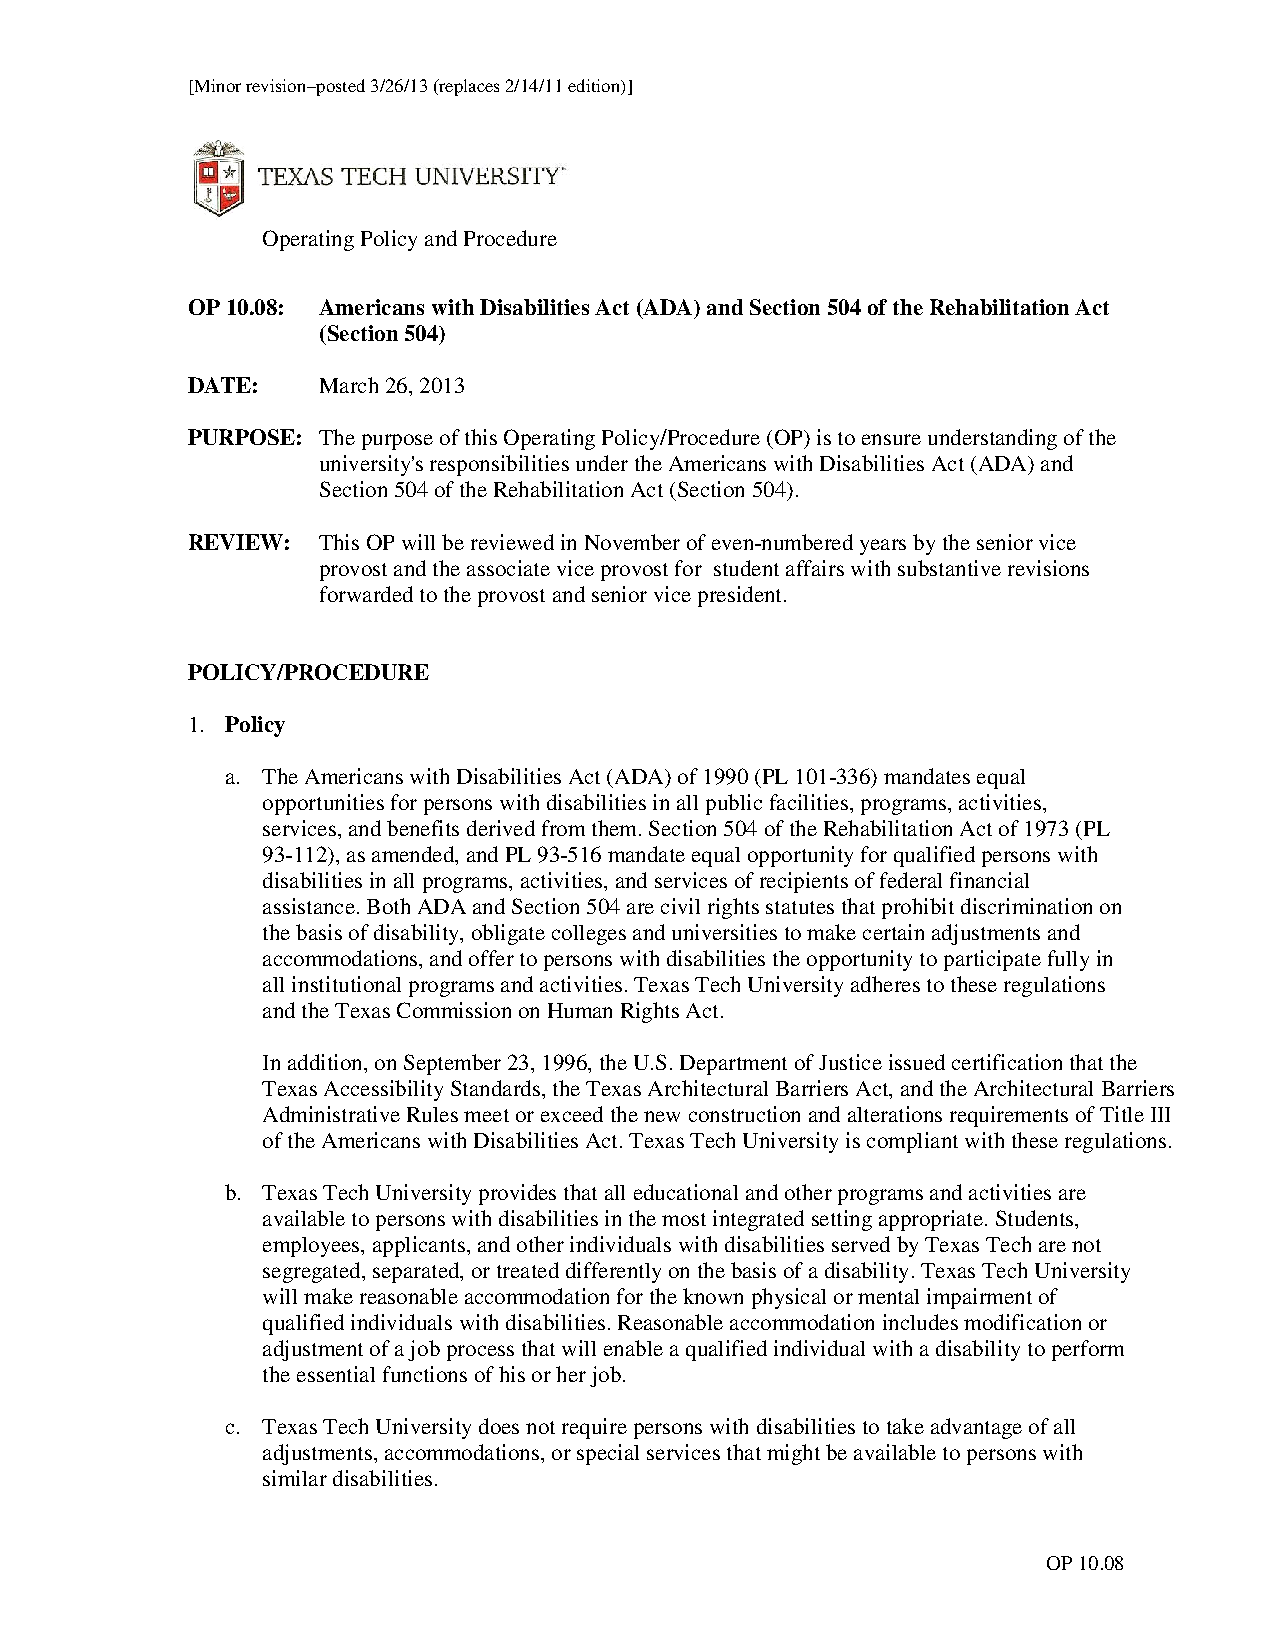
\includepdf[pages=-]{./OP10-08.pdf}
%\bibitem[\protect\citeauthoryear{Gironas, Roesner, and Davis}{Gironas
% et~al.}{2009}]{gironas2009}
%Gironas, J., L.~A. Roesner, and J.~Davis (2009).
%\newblock {Storm Water Management Model} applications manual.
%\newblock Technical Report EPA/600/R-09/077, U.S. Environmental Protection
%  Agency, National Risk Management Research Laboratory Cincinnati, OH 45268.

\end{thebibliography}



\end{document}  

\bibitem[\protect\citeauthoryear{Chin}{Chin}{2006}]{Chin2006}
Chin, D. (2006). 
\newblock{\em Water Resources Engineering, 2 ed.}
\newblock Prentice Hall, Inc.

\bibitem[\protect\citeauthoryear{Mays}{Mays}{2011}]{mays2011}
Mays, L.~W. (2011).
\newblock {\em Water-Resources Engineering}.
\newblock Wiley.

\bibitem[\protect\citeauthoryear{Wurbs}{Wurbs}{2002}]{Wurbs2002}
Wurbs, R.A., and James, W. P. (2002).
\newblock{\em Water Resources Engineering}
\newblock Prentice Hall; pp.130-156; and 156-198. 

\bibitem[\protect\citeauthoryear{NCEES}{NCEES}{2008}]{ncees2008}
NCEES (2008).
\newblock {\em Fundamentals of Engineering Supplied Reference Handbook\/} (8th
  ed.).
\newblock 280 Seneca Creek Road, Clemson, SC 29631: National Council of
  Examiners for Engineering and Surveying {ISBN 978-1-932613-37-7}.

\bibitem[\protect\citeauthoryear{Roberson}{Roberson}{1988}]{roberson1988}
Roberson, J.~A., Cassidy, J. ~J., and Chaudry, M.~H.  (1988).
\newblock {\em Hydraulic Engineering}.
\newblock Houghton Mifflin.

\bibitem[\protect\citeauthoryear{Rossman}{Rossman}{2000}]{rossman2000}
Rossman, L. (2000).
\newblock {EPANET 2} users manual.
\newblock Technical Report EPA/600/R-00/057, U.S. Environmental Protection
  Agency, National Risk Management Research Laboratory Cincinnati, OH 45268.
  
\bibitem[\protect\citeauthoryear{Rossman}{Rossman}{2009}]{rossman2009}
Rossman, L. (2009).
\newblock {Storm Water Management Model} user's manual version 5.0.
\newblock Technical Report EPA/600/R-05/040, U.S. Environmental Protection
  Agency, National Risk Management Research Laboratory Cincinnati, OH 45268.